% -*- coding: utf-8 -*-
\documentclass[9pt]{beamer}

\usetheme[secheader]{Boadilla}
%\usepackage[french]{babel}
% use utf8 because bug with package circuitikz
\usepackage[utf8]{inputenc}

\usepackage{hyperref}
\usepackage{graphicx}
\usepackage{media9}
\usepackage{amsmath,amsthm,amsfonts}
\usepackage{pgfplots}
%\usepackage{theorem}

\title{}
\begin{document}

\begin{frame}{}
  \maketitle
\end{frame}

\section{Problem statement}

\begin{frame}{Eye description}
Eye is the organs of vision; it allows the conversion of light into impulses in neurons
\begin{center}
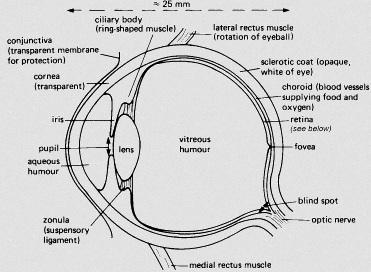
\includegraphics[width=.7\linewidth]{Eye.jpg}
\end{center}
\tiny{source: \url{http://academia.hixie.ch/bath/eye/home.html}}
\end{frame}

\begin{frame}{Eye description}
Aqueous humor is produced by the ciliary epithelium and drains into the Schlemm's canal and the pressure produced is the intra-ocular pression.
\begin{center}
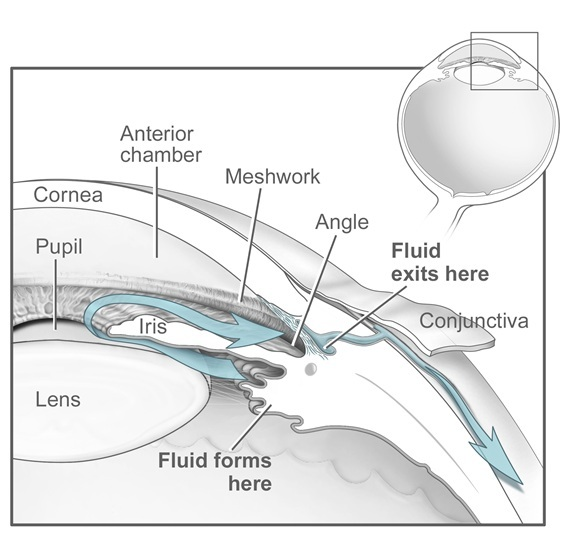
\includegraphics[width=.5\linewidth]{Humor.jpg}
\end{center}


\end{frame}

\begin{frame}{IOP}
The IOP range between 10 and 22 mmHg for human with an average value of 16 mmHg.
It also inflates the globe of the eye

Note that its value can be measured by tonometry by taking into account the thickness of the cornea. A fine jet of air is directed toward the cornea.
\begin{center}
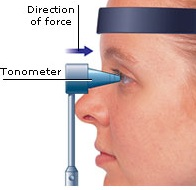
\includegraphics[scale=.6]{Tonometry.jpg}\\
\tiny{source: \url{http://www.aviva.co.uk/health-insurance/home-of-health/medical-centre/medical-encyclopedia/entry/test-tonometry/}}
\end{center}
Problems begin with an elevated IOP which is a major risk factor for glaucoma.
\end{frame}

\begin{frame}{Glaucoma}
The glaucoma, also called the silent thief of sight, is known as the second leading cause of blindness worldwide (1 in 40 adults over 40 years old).
\newline
\\
 Until now, the major risk for glaucoma is the elevated IOP but it is neither required nor enough to actually contract the disease:\\
-a patient could have a glaucoma with a low IOP\\
-a patient with an elevated IOP may never contracts glaucoma. 
As a matter of fact, 25 \% of IOP-treated patient progress to blindness.

\end{frame}

\begin{frame}
This disease can be described as a group of ocular disorders with multi-factorial etiology united by a clinically characteristic optic neuropathy accompanied by a vision loss.
\newline
\\
There are two kinds of diagnostics: \\
-a morphological damage (optic disk damage)
\begin{center}
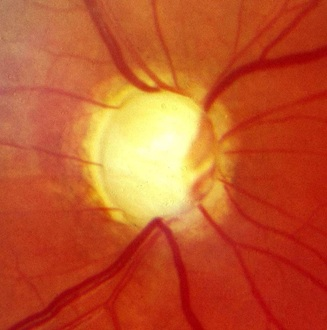
\includegraphics[scale=.5]{Morphological.jpg}\\
\tiny{Glaucomateous optic nervehead demonstrating increased cup to disc ratio}
\end{center}
Description of the picture ...
\end{frame}
\begin{frame}
-a physiological damage (decrease of the visual field)
\begin{center}
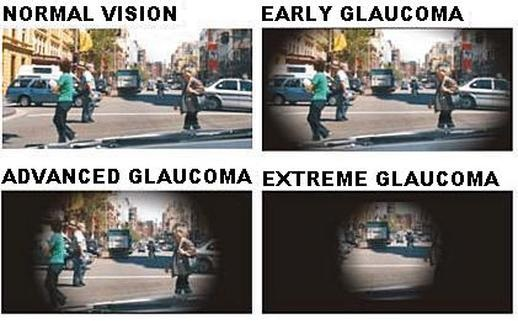
\includegraphics[scale=.5]{Glaucoma.jpg}\\
\tiny{source: \url{http://www.swisscompleteeyecare.com/uploads/3/6/3/8/3638142/8901258.jpg?520}}

\end{center}

However, the IOP remains the only parameter we can act on, either by surgery or with medications.
\end{frame}

\begin{frame}{Treatment}

The medications have two effects: either decrease the secretion of aqueous humor or increase the elimination of it. It is also possible to combine several treatments in order to decrease even more the IOP.
\newline
\\
\begin{tabular}{|c|c|}
\hline
Decrease the secretion of aqueous humor & Increase the elimination of aqueous humor\\
\hline
beta-adrenergic receptor antagonists & Prostaglandin analogs \\
Alpha2-adrenergic agonists & Miotic agents \\
alpha agonists &  \\
Carbonic anhydrase inhibitors &  \\
\hline
\end{tabular}
\newline
\newline
Beside, drugs could work better on patients depending on their age, gender, ethnic group, other diseases like diabetes, hypertension. 

\end{frame}

\section{Mathematical Model}

\begin{frame}{Model of intraocular fluids dynamics}
$$ \frac{dU}{dt}=F_{h}-F_{e}$$
$U$: Total aqueous humor\\
$F_h$: Fluid inflow in posterior chamber\\
$F_e$: net inflow via trabecular path
\newline
\\

$$F_{h}= L_p \big[ (p_a-p)-\sigma_{p} \Delta\pi_{p}-\sigma_{s} \Delta\pi_{s}\big]$$\\
$L_p$: permeability of the equivalent membrane\\
$p_a$: pressure in the ciliary body capillaries\\
$p$: IOP \\
$\sigma_p$: reflection coefficient (proteins)\\
$\sigma_s$: reflection coefficient (low molecular components)\\
$\Delta \pi_p $: osmotic pressure diff. accross membrane (proteins)\\
$\Delta \pi_s $: osmotic pressure diff. across membrane (low molecular component)
\newline
\\
\end{frame}
\begin{frame}
$$\Delta\pi_{s}= \rho(C_1-C_{2}) $$\\
$\rho$ & universal gas constant $\times$  absolute temperature\\
$C_1$: total molar concentration of low-molecular components (blood)\\
$C_2$: total molar concentration of low-molecular components (intra-ocular fluid near ciliary body surface) 
\newline
\\
$$ V^{\ast} \frac{dC_{2}}{dt}= Q_s-Q_e=\xi_s(C_1-C_{2})+F_h (1-\sigma_s) \bar{C}+J-F_h C_2$$\\
$V^\star$: volume of intraocular fluid between the folds of the ciliary body\\
$\xi_s$: average permeability of membrane for low-molecular species\\
$\overline{C}$=$\displaystyle{\frac{C_1+C_2}{2}}$\\
$J$: Influx due to active transport
\newline
\\
$$ \alpha \frac{dp}{dt}=F_{h}-\frac{p-p_e}{R}$$\\
$p_e$: pressure in the episcleral veins\\
$R$: output hydraulic resistance\\
$\alpha$: volume compliance of the eye shell (varies significantly)
\newline
\\
\end{frame}

\begin{frame}{Assumptions}

\end{frame}

\begin{frame}{Data}

\end{frame}

\section{Numerical Results}

\begin{frame}{Recovering some values}
%\pgfplotsset{
%  compat=newest,
%  xlabel near ticks,
%  ylabel near ticks
%}
\end{frame}

\begin{frame}{Summary}
-3 equations
\end{frame}

\end{document}



%%% Local Variables:
%%% coding: utf-8
%%% mode: latex
%%% TeX-PDF-mode: t
%%% TeX-parse-self: t
%%% x-symbol-8bits: nil
%%% TeX-auto-regexp-list: TeX-auto-full-regexp-list
%%% TeX-master: t
%%% ispell-local-dictionary: "american"
%%% End:
